\scanpage{65}
\mspage{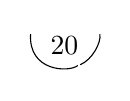
\begin{tikzpicture}[baseline=(n.base)]\node (n) at (0,0) {20};\draw (-.43,.15) .. controls (-.46,-.33) and (.06,-.34) .. (.17,-.25);\draw (.20,-.24) .. controls (.35,-.18) and (.47,.04) .. (.45,.15);\end{tikzpicture}}

These are also the \deleted{diagrams} solid-line arrows of the fundamental diagram (17)

With the ordered set $I$, let us therefore make a \deleted{ordered set} \uline{diagram} whose vertices are \deleted{``letters'' $\unsure{x|i}\ i^*$} symbols \deleted{$i_{**}$} $[i]$, $[i,j]$, $[i,j]^*$, where $i,j\in I$, $j$ a successor of $i$. The arrows of the diagram are \unsure{of the|of} three types which are all described in
\diagram{$(19)\qquad$\begin{tikzcd}[column sep=large,row sep=large]
{[i,j]^*} \arrow[r] \arrow[d] & {[i,j]} & i^* \arrow[l] \\
{[j]^*} & &
\end{tikzcd}}

Let us denote by $\widetilde I$ this diagram, whose set of vertices \deleted{is identified} \unsure{with|has} \deleted{$\unsure{I\times I_\Delta}$} \inserted{cardinality} $\operatorname{card}I+2\nu$ \deleted{\unsure{cardinality}} \inserted{where $\nu=\operatorname{card}$} of the set of ``elementary'' flags $(i<j)$ \inserted{i.e. such that $j$ is a successor of $i$} and the number of arrows is $3\nu$. If $I$ contains \unsure{exactly|exactly} two elements $i,j$ with $i<j$, \inserted{i.e. $I\simeq\Delta_1$,} this diagram is en. (19). If $I=\Delta_r=(0,1,\ldots,r)$, one finds (now using the symbols for the $X_i^*,V_{ij}^*,V_{ij}$ which realize the diagram)

\margin{64}
